\documentclass[a4paper]{scrreprt}

\usepackage[ngerman]{babel}
\usepackage[utf8]{inputenc}
\usepackage[T1]{fontenc}
\usepackage{ae}
\usepackage[bookmarks, bookmarksnumbered]{hyperref}
\usepackage{tabularx}
\usepackage{graphicx}
\usepackage{csquotes}
\usepackage{verbatim}
\usepackage[nonumberlist, toc, section]{glossaries}
\usepackage[german]{fancyref}

\makeglossaries

\setcounter{secnumdepth}{3}


% Document
% zu jedem umgesetzten Punkt des Pflichtenhefts Bezug herstellen

\begin{document}

    \tableofcontents
    \chapter{Einleitung}
    \chapter{Architekturdiagramm}

    \chapter{Klassendiagramme}
    \section{API}
    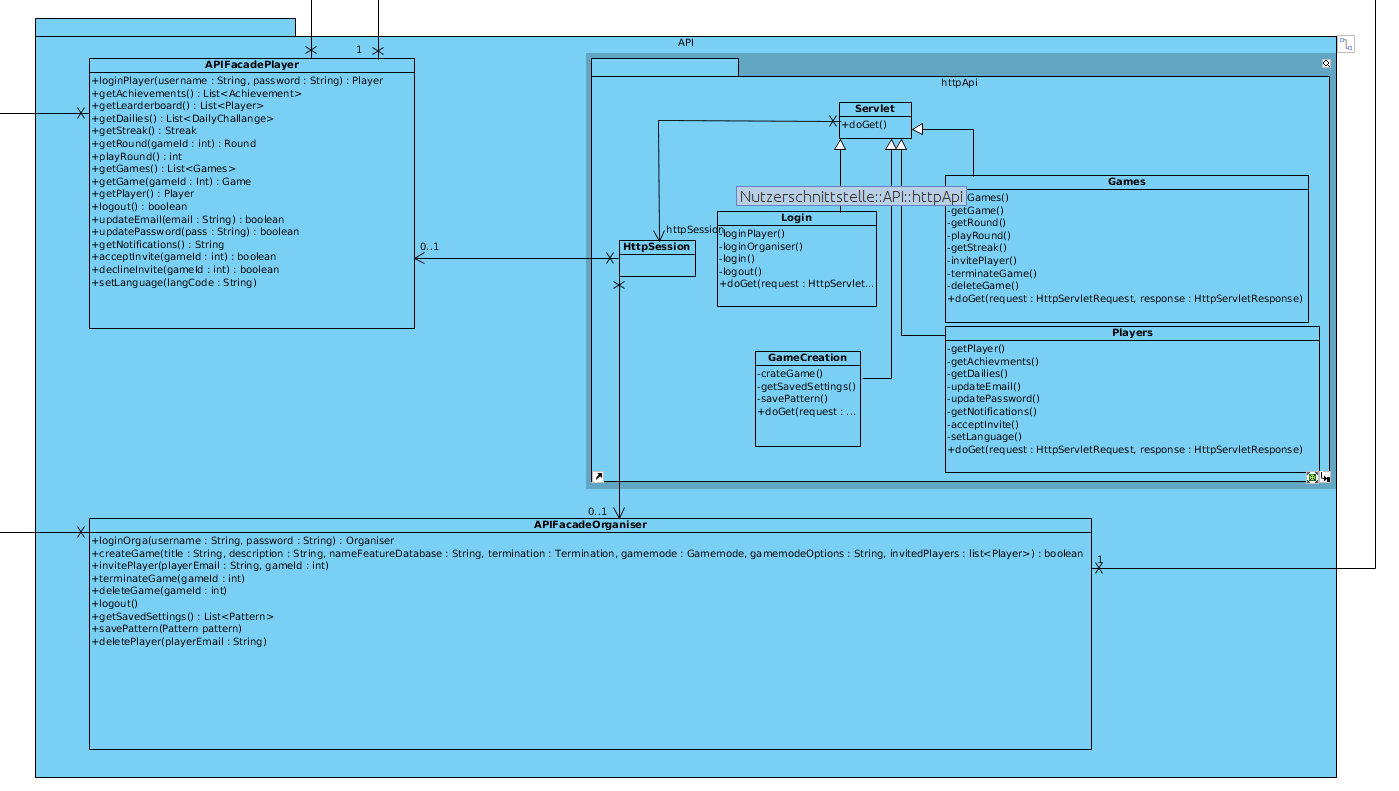
\includegraphics[width=\textwidth]{img/api.png}
    \subsection{APIFacadePlayer}
        Eine APIFacadePlayer ist das Objekt, über welches sämtliche Interaktion mit dem System von den Spielern aus passiert. Nach dem Konstruktor \textbf{muss} zuerst loginPlayer aufgerufen werden, bis es erfolgreich zurückkehrt. Ansonsten haben alle anderen Methoden kein definiertes Verhalten und werden im Allgemeinem nichts nützliches zurückgeben. Eine APIFacadePlayer ist immer mit einem Spieler assoziert, falls dieser korrekt angemeldet wurde. Alle Methoden beziehen sich dann auf den angemeldeten Spieler.
    \subsubsection{loginPlayer}
        \begin{itemize}
            \item Beschreibung: Versucht einen Spieler mit email und password anzumelden. Bei Erfolg wird diese Facade mit dem Spieler assoziert.
            \item Parameters: 
                \begin{itemize}
                    \item email: Die Email Adresse mit der eine Anmeldung versucht wird
                    \item password: Das Passwort zu mit dem eine Anmeldung versucht wird
                \end{itemize}
            \item Rückgabewert: Falls die Email-Passwort Kombination einen validen Spieler beschreibt, wird dieser zurückgegeben. Andernfalls wird null zurückgegeben.
        \end{itemize}
    \subsubsection{logout}
    \begin{itemize}
        \item Beschreibung: Meldet den angemeldeten Spieler ab. Nach dem Aufruf dieser Methode verhält sich dieses Objekt wieder so, als ob nie ein Spieler angemeldet wurde
    \end{itemize}
    \subsubsection{getAchievments}
    \begin{itemize}
        \item Beschreibung: Holt die Liste aller Achievments, mit der Information ob der Spieler diese bereits erreicht hat oder nicht.
        \item Rückgabewert: Liste an Achievments. 
    \end{itemize}
    \subsubsection{getLeaderboard}
    \begin{itemize}
        \item Beschreibung: Gibt das aktuelle Leaderboard in der geordneten Reihenfolge zurück
        \item Rückgabewert: Eine Liste an Spielern, geordnet nach ihrer Leaderboard-Ordunung. 
    \end{itemize}
    \subsubsection{getDailies}
    \begin{itemize}
        \item Beschreibung: Gibt die Daily-Challenges für diesen Spieler zurück, mit der Information, wie weit diese bereits erfüllt sind.
        \item Rückgabewert: Eine Liste an Daily-Challenges für diesen Spieler mit Information, wie weit diese erfüllt sind.
    \end{itemize}
    \subsubsection{getStreak}
    \begin{itemize}
        \item Beschreibung: Gibt das aktuelle Streak-Objekt für diesen Spieler zurück
        \item Rückgabewert: Das aktuelle Streak-Objekt für diesen Spieler 
    \end{itemize}
    \subsubsection{getPoints}
    \begin{itemize}
        \item Beschreibung: Gibt die Punkte des Spielers zurück
        \item Rückgabewert: Aktuelle Punktzahl des Spielers 
    \end{itemize}
    \subsubsection{getRound}
    \begin{itemize}
        \item Beschreibung: Fordert die nächste Runde für ein Spiel an und gibt diese zurück
        \item Parameter:
        \begin{itemize}
            \item gameId: Eindeutige Id des Spieles für das die Runde angefordert wird
        \end{itemize}
        \item Rückgabewert: Wenn der Spieler eine Runde in dem angegebenem Spiel spielen darf, dann wird das Runden-Objekt zurückgegen. Andernfalls wird null zurückgegeben 
    \end{itemize}
    \subsubsection{playRound}
    \begin{itemize}
        \item Beschreibung: Spielt eine Runde in der aktuellen Runde
    \end{itemize}
    \subsubsection{getGames}
    \begin{itemize}
        \item Beschreibung: Holt alle Spiele, an denen der Spieler teilnimmt
        \item Rückgabewert: Liste an Spielen, an denen der Spieler teilnimmt 
    \end{itemize}
    \subsubsection{getGame}
    \begin{itemize}
        \item Beschreibung: Gibt ein Spiel nach Id zurück, falls der Spieler auf dieses Spiel Zugriff hat
        \item Parameter:
        \begin{itemize}
            \item gameId: die Id des Spiels, welches zurückgegeben werden soll
        \end{itemize}
        \item Rückgabewert: Falls gameId valid ist, also Spiel existiert und Spieler darf auf das Spiel zugreifen, dann wird das Spiel zurückgegen, ansonsten null. 
    \end{itemize}
    \subsubsection{getPlayer}
    \begin{itemize}
        \item Beschreibung: Gibt den angemeldeten Spieler zurück. Also der Spieler, welcher durch loginPlayer angemeldet wurde.
        \item Rückgabewert: Der angemeldete Spieler, falls keiner angemeldet ist wird null zurückgegeben. 
    \end{itemize}
    \subsubsection{updateEmail}
    \begin{itemize}
        \item Beschreibung: Ändert die E-Mail-Adresse mit der sich ein Spieler anmeldet. Die Änderung tritt erst in Effekt, wenn die neue Email-Adresse bestätigt wurde.
        \item Parameter:
        \begin{itemize}
            \item email: Die neue E-Mail-Adresse, welche in Zukunft für diesen Spieler verwendet werden soll.
        \end{itemize}
        \item Rückgabewert: true falls die Bestätigungsemail veschickt wurde, false andernfalls 
    \end{itemize}
    \subsubsection{updatePassword}
    \begin{itemize}
        \item Beschreibung: Ändert das Passwort mit dem sich der Spieler anmeldet. Die Änderung tritt sofort in Effekt.
        \item Parameter:
        \begin{itemize}
            \item pass: Das neue Passwort
        \end{itemize}
        \item Rückgabewert: true falls die Änderung erfolgreich war, false andernfalls 
    \end{itemize}
    \subsubsection{getNotifications}
    \begin{itemize}
        \item Beschreibung: Holt alle Notifications, die für diesen Spieler anliegen
        \item Rückgabewert:  Alle Notifications, die für diesen Spieler anliegen
    \end{itemize}
    \subsubsection{acceptInvite}
    \begin{itemize}
        \item Beschreibung: Akzeptiert eine Einladung zu einem Spiel, welche diesem Spieler geschickt wurde und löscht diese aus seinen Einladungen
        \item Parameter:
        \begin{itemize}
            \item gameId: Id des Spiels für das die Einladung angenommen werden soll.
        \end{itemize}
        \item Rückgabewert: true wenn die Einladung angenommen wurde, false falls der Spieler keine Einladung zu diesem Spiel hatte, das Spiel nicht existier oder bereits beendet ist. 
    \end{itemize}
    \subsubsection{declineInvite}
    \begin{itemize}
        \item Beschreibung: Lehnt eine Einladung zu einem Spiel ab, welche diesem Spieler geschickt wurde und löscht diese aus seinen Einladungen
        \item Parameter:
        \begin{itemize}
            \item gameId: Id des Spiels für das die Einladung abgelehnt werden soll.
        \end{itemize}
        \item Rückgabewert: true wenn die Einladung abgelehnt wurde, false falls der Spieler keine Einladung zu diesem Spiel hatte, das Spiel nicht existier oder bereits beendet ist. 
    \end{itemize}
    \subsubsection{setLanguage}
    \begin{itemize}
        \item Beschreibung: Setzt die Sprache für den Spieler
        \item Parameter:
        \begin{itemize}
            \item langCode: der Landescode für die gewünschte Sprache
        \end{itemize}
    \end{itemize}
    \subsection{APIFacadeOrganiser}
    \subsubsection{loginOrganiser}
    \begin{itemize}
        \item Beschreibung: meldet einen Organisator an. Damit dies möglich ist, muss der Organisator vorher registriert worden sein.
        \item Parameter:
        \begin{itemize}
            \item email: E-Mail des anzumeldenden Organisators
            \item password: Das Passwort des anzumeldenden Organisators
        \end{itemize}
        \item Rückgabewert: Falls die Email-Passwort Kombinnation valid ist, also ein Organisator mit der E-Mail registriert ist und das Passwort ist richtig, wird der Organisator zurückgegeben. Andernfalls null. 
    \end{itemize}
    \subsubsection{createGame}
    \begin{itemize}
        \item Beschreibung: erstellt ein Spiel für diesen Organisator.
        \item Parameter: %% stuff bleibt hier ja noch nicht ganz fest gegeben
        \begin{itemize}
            \item :
        \end{itemize}
        \item Rückgabewert: Falls das Erstellen erfolgreich war, true zurückgegeben, andernfalls false. 
    \end{itemize}
    \subsubsection{invitePlayer}
    \begin{itemize}
        \item Beschreibung: Lädt einen Spieler zu einem Spiel des Organisators ein.
        \item Parameter:
        \begin{itemize}
            \item playerEmail: die Email-Adresse des einzuladenden Spielers
            \item gameId: Das Spiel, zu dem der Spieler eingeladen werden soll. Das Spiel muss ein Spiel des Organisators sein.
        \end{itemize}
    \end{itemize}
    \subsubsection{terminateGame}
    \begin{itemize}
        \item Beschreibung: Beendet ein Spiel des Organisators. 
        \item Parameter:
        \begin{itemize}
            \item gameId: Id des zu beendenden Spiels. Das Spiel muss zu dem Organisator gehören.
        \end{itemize}
    \end{itemize}
    \subsubsection{deleteGame}
    \begin{itemize}
        \item Beschreibung: Löscht ein Spiel des Organisators aus dem System. 
        \item Parameter:
        \begin{itemize}
            \item gameId: Die Id des zu löschende Spiel
        \end{itemize}
    \end{itemize}
    \subsubsection{logout}
    \begin{itemize}
        \item Beschreibung: Meldet einen Organisator ab. Nach dem Aufruf dieser Methode verhält sich dieses Objekt so, als ob niemand angemeldet war.
    \end{itemize}
    \subsubsection{getSavedSettings}
    \begin{itemize}
        \item Beschreibung: Holt eine Liste aller gespeicherten Einstellungen dieses Organisators.
        \item Rückgabewert: Eine Liste aller gespeichterten Einstellungen dieses Organisators. 
    \end{itemize}
    \subsubsection{savePattern}
    \begin{itemize}
        \item Beschreibung: Speichert eine Einstellungskonfiguration für diesen Organisator
        \item Parameter:
        \begin{itemize}
            \item pattern: Das zu speichernde Pattern
        \end{itemize}
    \end{itemize}

    \begin{comment} Vollständiges Doku-Template
    \begin{itemize}
        \item Beschreibung:
        \item Parameter:
        \begin{itemize}
        \end{itemize}
        \item Rückgabewert:
    \end{itemize}
    \end{comment}

    \section{Database}
    Paket das die Kommunikation mit der Datenbank übernimmt.

    \subsection{DatabaseAdapter}
    Abstrakte Klasse die als Singleton realisiert ist und von der jeweiligen Datenbankimplementierung abstrahiert.

    \subsubsection{instance}
    Instanz des Singletons die durch Vererbung spezialisiert wird.

    \subsubsection{getInstance}
    \begin{itemize}
        \item Beschreibung: Statische Methode die die Instanz des DatabaseAdapters zurückgibt
        \item Rückgabewert: Instanz des DatabaseAdapters
    \end{itemize}

    \subsubsection{getPlayerAdapter}
    \begin{itemize}
        \item Beschreibung: Gibt den PlayerAdapter für den Spieler mit der gegebenen ID zurück.
        \item Parameter:
        \begin{itemize}
            \item id: ID des Spielers, dessen PlayerAdapter zurückgegeben werden soll.
        \end{itemize}
        \item Rückgabewert: PlayerAdapter des Spielers mit ID id.
    \end{itemize}

    \subsubsection{getOrganiserAdapter}
    \begin{itemize}
        \item Beschreibung: Gibt den OrganiserAdapter für den Organisator mit der gegebenen ID zurück.
        \item Parameter:
        \begin{itemize}
            \item id: ID des Organisators, dessen OrganiserAdapter zurückgegeben werden soll.
        \end{itemize}
        \item Rückgabewert: OrganiserAdapter des Organisators mit ID id.
    \end{itemize}

    \subsubsection{getGameAdapter}
    \begin{itemize}
        \item Beschreibung: Gibt den GameAdapter für das Spiel mit der gegebenen ID zurück.
        \item Parameter:
        \begin{itemize}
            \item id: ID des Spiels, dessen GameAdapter zurückgegeben werden soll.
        \end{itemize}
        \item Rückgabewert: GameAdapter des Spiels mit ID id.
    \end{itemize}

    \subsection{UserAdapter}
    Schnittstelle die Methoden für alle Nutzer des Produkts bereitstellt.
    Jeder UserAdapter ist genau einem Nutzer zugeordnet.

    \subsubsection{getID}
    \begin{itemize}
        \item Beschreibung: Gibt die ID des Nutzers zurück.
        \item Rückgabewert: int mit ID des Nutzers.
    \end{itemize}

    \subsubsection{getEmail}
    \begin{itemize}
        \item Beschreibung: Gibt die E-Mail-Addresse des Nutzers zurück.
        \item Rückgabewert: String mit E-Mail-Addresse des Nutzers.
    \end{itemize}

    \subsubsection{getUsername}
    \begin{itemize}
        \item Beschreibung: Gibt den Nutzernamen des Nutzers zurück.
        \item Rückgabewert: String mit Nutzernamen des Nutzers.
    \end{itemize}

    \subsubsection{getPasswordHash}
    \begin{itemize}
        \item Beschreibung: Gibt das gehashte Passwort des Nutzers zurück.
        \item Rückgabewert: Hash des Passworts
    \end{itemize}

    \subsubsection{setEmail}
    \begin{itemize}
        \item Beschreibung: Setzt die E-Mail-Addresse des Nutzers neu.
        \item Parameter:
        \begin{itemize}
            \item email: String der neuen E-Mail-Addresse.
        \end{itemize}
    \end{itemize}

    \subsubsection{setPasswordHash}
    \begin{itemize}
        \item Beschreibung: Setzt das gehashte Passwort des Nutzers neu.
        \item Parameter:
        \begin{itemize}
            \item hash: Hash des neuen Passworts
        \end{itemize}
    \end{itemize}

    \subsection{PlayerAdapter}
    Schnittstelle die UserAdapter erweitert.
    Jeder PlayerAdapter ist stets genau einem Spieler zugeordnet.

    \subsubsection{getPlayerStats}
    \begin{itemize}
        \item Beschreibung: Gibt die gespeicherten PlayerStats eines Spielers zurück.
        \item Rückgabewert: PlayerStats Objekt des Spielers.
    \end{itemize}

    \subsection{OrganiserAdapter}
    Schnittstelle die UserAdapter erweitert.
    Jeder OrganiserAdapter ist stets genau einem Organisator zugeordnet.

    \subsubsection{getPatterns}
    \begin{itemize}
        \item Beschreibung: Gibt die gespeicherten Patterns des Organisators zurück.
        \item Rückgabewert: Collection der gespeicherten Patterns des Organisators.
    \end{itemize}

    \subsection{GameAdapter}
    Schnittstelle die Methoden für gespeicherte Spiele des Produkts bereitstellt.
    Jeder GameAdapter ist stets genau einem Spiel zugeordnet.

    \subsubsection{getTitle}
    \begin{itemize}
        \item Beschreibung: Gibt den Titel des Spiels zurück.
        \item Rückgabewert: String mit Titel.
    \end{itemize}

    \subsubsection{getDescription}
    \begin{itemize}
        \item Beschreibung: Gibt die Beschreibung des Spiels zurück.
        \item Rückgabewert: String mit Beschreibung des Spiels.
    \end{itemize}

    \subsubsection{getDatabaseName}
    \begin{itemize}
        \item Beschreibung: Gibt den Namen der Datenbank zurück in der das Spiel gespeichert ist.
        \item Rückgabewert: String mit Namen der Datenbank.
    \end{itemize}

    \subsubsection{getFeatures}
    \begin{itemize}
        \item Beschreibung: Gibt die Features des Spiels zurück.
        \item Rückgabewert: Collection mit den Features des Spiels.
    \end{itemize}

    \subsubsection{getNumberOfRounds}
    \begin{itemize}
        \item Beschreibung: Gibt die Anzahl der zu spielenden Runden zurück.
        \item Rückgabewert: int mit zu spielenden Runden.
    \end{itemize}

    \subsubsection{getInvitedPlayers}
    \begin{itemize}
        \item Beschreibung: Gibt die eingeladenen Spieler zurück.
        \item Rückgabewert: Collection mit den eingeladenen Spielern
    \end{itemize}

    \subsubsection{getPlayingPlayers}
    \begin{itemize}
        \item Beschreibung: Gibt die spielenden Spieler zurück.
        \item Rückgabewert: Collection mit den spielenden Spielern.
    \end{itemize}

    \subsubsection{getRounds}
    \begin{itemize}
        \item Beschreibung: Gibt die gespielten Runden zurück.
        \item Rückgabewert: Collection der gespielten Runden.
    \end{itemize}

    \subsubsection{getGamemode}
    \begin{itemize}
        \item Beschreibung: Gibt den gewählten Spielmodus zurück.
        \item Rückgabewert: Gamemode
    \end{itemize}

    \subsubsection{getTermination}
    \begin{itemize}
        \item Beschreibung: Gibt die Art der Spielterminierung zurück.
        \item Rückgabewert: Termination
    \end{itemize}

    \subsubsection{isFinished}
    \begin{itemize}
        \item Beschreibung: Gibt zurück ob das Spiel beendet wurde oder nicht.
        \item Rückgabewert: True falls das Spiel beendet wurde, false sonst
    \end{itemize}

    \subsubsection{addPlayer}
    \begin{itemize}
        \item Beschreibung: Fügt einen Spieler zum Spiel hinzu.
        \item Parameter:
        \begin{itemize}
            \item player: Spieler der hinzugefügt werden soll.
        \end{itemize}
    \end{itemize}

    \subsubsection{addRound}
    \begin{itemize}
        \item Beschreibung: Fügt eine Runde zum Spiel hinzu.
        \item Parameter:
        \begin{itemize}
            \item round: Runde die hinzugefügt werden soll.
        \end{itemize}
    \end{itemize}

    \subsubsection{setTermination}
    \begin{itemize}
        \item Beschreibung: Setzt die Art der Spielterminierung.
        \item Parameter:
        \begin{itemize}
            \item termination: Termination Objekt das die Art der Spielterminierung festlegt.
        \end{itemize}
    \end{itemize}

    \subsubsection{setFeatures}
    \begin{itemize}
        \item Beschreibung: Setzt die Features des Spiels.
        \item Parameter:
        \begin{itemize}
            \item features: Collection mit den Features des Spiels.
        \end{itemize}
    \end{itemize}


    \subsection{Mysql}
    Paket mit Mysql basierter Implementierung der Datenbank.
    Mitgelieferte Standard-Implementierung des Produkts.

    \subsubsection{MysqlDatabaseAdapter}
    Mysql Implementierung der DatabaseAdapter Klasse.

    \subsubsection{MysqlUserAdapter}
    Mysql Implementierung der UserAdapter Schnittstelle.

    \subsubsection{MysqlPlayerAdapter}
    Mysql Implementierung der PlayerAdapter Schnittstelle.
    Erbt von MysqlUserAdapter

    \subsubsection{MysqlOrganiserAdapter}
    Mysql Implementierung der OrganiserAdapter Schnittstelle.
    Erbt von MysqlUserAdapter

    \subsubsection{MysqlGameAdapter}
    Mysql Implementierung der GameAdapter Schnittstelle.

    \section{Configuration}
    Paket für die Kommunikation mit der Konfigurationsdatei.

    \subsection{Configuration}
    Abstrakte Klasse die von der Config-Implementierung abstrahiert.
    Kümmert sich um die Kommunikation des Produkts mit der Konfigurationsdatei.
    Ist als Singleton umgesetzt um zu erzwingen, dass stets nur ein Zugriffspunkt zur Konfiguration besteht.

    \subsubsection{getInstance}
    \begin{itemize}
        \item Beschreibung: Statische Methode die die Instanz der Configuration zurückgibt.
        \item Rückgabewert: Instanz der Configuration.
    \end{itemize}


    \subsubsection{getOrganiserPassword}
    \begin{itemize}
        \item Beschreibung: Gibt das Passwort als String zurück das Organisatoren bei der Erstregistrierung verwenden müssen.
        \item Rückgabewert: String mit Organisatorpasswort
    \end{itemize}

    \subsubsection{getMLServerURL}
    \begin{itemize}
        \item Beschreibung: Gibt die URL als String zurück, unter der der ML-Server zu finden ist
        \item Rückgabewert: String mit URL des ML-Servers
    \end{itemize}

    \subsubsection{getDatabaseType}
    \begin{itemize}
        \item Beschreibung: Gibt die Art der verwendeten Datenbankimplementierung zurück.
        \item Rückgabewert: String mit Name der Datenbankimplementierung.
    \end{itemize}

    \subsubsection{getDatabaseHostname}
    \begin{itemize}
        \item Beschreibung: Gibt den Hostnamen des Datenbankservers zurück.
        \item Rückgabewert: String mit Hostnamen des Datenbankservers.
    \end{itemize}

    \subsubsection{getDatabasePort}
    \begin{itemize}
        \item Beschreibung: Gibt den Port des Datenbankservers zurück.
        \item Rückgabewert: int mit Port des Datenbankservers.
    \end{itemize}

    \subsubsection{getDatabaseUsername}
    \begin{itemize}
        \item Beschreibung: Gibt den Nutzernamen mit dem sich am Datenbankserver angemeldet wird zurück.
        \item Rückgabewert: String mit Nutzernamen
    \end{itemize}

    \subsubsection{getDatabasePassword}
    \begin{itemize}
        \item Beschreibung: Gibt das Passwort mit dem sich am Datenbankserver angemeldet wird zurück.
        \item Rückgabewert: String mit Passwort
    \end{itemize}

    \subsection{DefaultConfiguration}
    Implementiert die abstrakte Klasse Configuration und stellt die Funktionalität bereit.
    Mitgelieferte Standardimplementierung der Konfiguration.

    \section{MLServer}
    Paket für die Kommunikation mit dem ML-Server.

    \subsection{MLServer}
    Abstrakte Klasse die von der Implementierung der ML-Server-API abstrahiert.
    Ist als Singleton umgesetzt um zu erzwingen dass stets nur ein Zugriffspunkt zum ML-Server existiert.

    \subsubsection{getInstance}
    \begin{itemize}
        \item Beschreibung: Statische Methode die die Instanz des MLServers zurückgibt.
        \item Rückgabewert: Instanz des MLServers.
    \end{itemize}

    \subsubsection{getVersion}
    \begin{itemize}
        \item Beschreibung: Gibt die Version des genutzten ML-Servers als String zurück.
        \item Rückgabewert: String mit der Versionsnummer.
    \end{itemize}

    \subsubsection{getFeatures}
    \begin{itemize}
        \item Beschreibung: Gibt die Features des angegebenen Datensatzes zurück
        \item Parameter:
            \begin{itemize}
                \item dataset: Datensatz dessen Features zurückgegeben werden sollen.
            \end{itemize}
        \item Rückgabewert: Collection mit den Features des Datensatzes.
    \end{itemize}

    \subsubsection{getScore}
    \begin{itemize}
        \item Beschreibung: Gibt die Bewertung der gesendeten Features zurück.
        \item Parameter:
            \begin{itemize}
                \item dataset: Datensatz von dem eine Merkmalsauswahl geschickt wird.
                \item selectedFeatures: Ausgewählte Merkmale.
            \end{itemize}
        \item Rückgabewert: double mit Wert im Intervall [0,1] der die Güte der Auswahl beschreibt.
    \end{itemize}

    \subsection{RESTMLServer}
    Implementiert die abstrakte Klasse MLServer und stellt die Funktionalität mittels der Standard-Implementierung des ML-Servers per REST-API bereit.
    
    
   \section{Gamification}
   %Insert Picture
   Paket für die Gamification-Elemente. Dazu gehören Punkte, Streak, Leaderboard, Achievements und Daily-Challenges.
   
   
   \subsection{Streak}
   Stellt eine Streak dar.
   
   \subsubsection{Streak}
   \begin{itemize}
   	  \item Beschreibung: Der Konstruktor einer Streak initialisiert den Zähler der Streak auf 0.
   \end{itemize}
   \subsubsection{setZero}
   \begin{itemize}
   	\item Beschreibung: Setzt den Zähler der Streak auf den Wert 0 zurück.
   \end{itemize}
   \subsubsection{increaseStreak}
   \begin{itemize}
   	\item Beschreibung: Erhöht den Zähler der Streak um den Wert 1.
   \end{itemize}
   \subsubsection{getCounter}
   \begin{itemize}
   	\item Beschreibung: Gibt den aktuellen Zähler zurück.
   	\item Rückgabewert: Der aktuelle Wert des Zählers.
   \end{itemize}
   
   
   \subsection{Leaderboard}
   Stellt ein Leaderboard dar.
   
   \subsubsection{getPlayers}
   \begin{itemize}
   	\item Beschreibung: Sortiert die Liste aus Spielern und gibt diese zurück.
   	\item Rückgabewert: Liste von Spielern.
   \end{itemize}
   \subsubsection{getInstance}
   \begin{itemize}
   	\item Beschreibung: Statische Methode. Sorgt dafür, dass nur ein LeaderBoard-Objekt existiert und gibt dieses zurück.
   	\item Rückgabewert: Das LeaderBoard-Objekt.
   \end{itemize}
   
   Das Paket Daylies enthält eine abstrakte Klasse DailyChallenge, von der alle konkreten Daily-Challenges erben.
   
   \subsection{DailyChallenge}
   Die abstrakte Klasse DailyChallenge gibt an, wie Daily-Challenges aufgebaut sind. Lediglich die Methode checkFinished() ist abstrakt und muss von den Unterklassen implementiert werden.
   \subsubsection{checkFinished}
   \begin{itemize}
     \item Beschreibung: Überprüft, ob die Aufgabe der Daily-Challenge erfüllt ist.
     \item Rückgabewert: True, wenn die Aufgabe erfüllt ist, sonst false.
    \end{itemize}
   \subsubsection{getCounter}
   \begin{itemize}
     \item Beschreibung: Gibt den Wert des aktuellen Zählers zurück.
     \item Rückgabewert: Der Werte des aktuellen Zählers.
    \end{itemize}
   \subsubsection{getName}
   \begin{itemize}
     \item Beschreibung: Gibt den Namen der Daily-Challenge zurück.
     \item Rückgabewert: Ein String vom Namen der Daily-Challenge.
    \end{itemize}
   \subsubsection{getDescription}
   \begin{itemize}
     \item Beschreibung: Gibt die Beschreibung der Daily-Challenge zurück.
     \item Rückgabewert: Ein String von der Beschreibung der Daily-Challenge.
    \end{itemize}
   \subsubsection{getReward}
   \begin{itemize}
   \item Beschreibung: Gibt die Beschreibung der Daily-Challenge zurück.
   \item Rückgabewert: Ein String von der Beschreibung der Daily-Challenge.
   \end{itemize}
   \subsubsection{getCounter}
   
   \subsection{DailyOne}
   Konkrete Implementierung der abstrakten Klasse DailyChallenge.
   \subsubsection{DailyOne}
   \begin{itemize}
   	\item Beschreibung: Der Konstruktor von DailyOne setzt Namen und Beschreibung von DailyOne und..
   	\item Parameter: Name und Beschreibung 
   \end{itemize}
   \subsubsection{checkFinished}
   %Konkret
   \subsubsection{getInstance}
   \begin{itemize}
   \item Beschreibung: Statische Methode. Sorgt dafür, dass nur ein DailyOne-Objekt existiert und gibt dieses zurück.
   \item Rückgabewert: Das DailyOne-Objekt.
   \end{itemize}
   
   \subsection{DailyTwo}
   Konkrete Implementierung der abstrakten Klasse DailyChallenge.
   \subsubsection{DailyTwo}
   \begin{itemize}
   	\item Beschreibung: Der Konstruktor von DailyTwo setzt Namen und Beschreibung von DailyTwo und..
   	\item Parameter: Name und Beschreibung 
   \end{itemize}
   \subsubsection{checkFinished}
   %Konkret
   \subsubsection{getInstance}
   \begin{itemize}
   \item Beschreibung: Statische Methode. Sorgt dafür, dass nur ein DailyTwo-Objekt existiert und gibt dieses zurück.
   \item Rückgabewert: Das DailyTwo-Objekt.
\end{itemize}
   
   Das Paket Achievements enthält eine abstrakte Klasse Achievement, von der alle konkreten Achievements erben.
   
   \subsection{Achievement}
   \subsubsection{isFinished}
   \begin{itemize}
   \item Beschreibung: Überprüft, ob die Aufgabe des Achievements erfüllt ist.
   \item Rückgabewert: True, wenn die Aufgabe erfüllt ist, sonst false.
\end{itemize}
   \subsubsection{getName}
   \begin{itemize}
   \item Beschreibung: Gibt den Namen des Achievements zurück.
   \item Rückgabewert: Ein String vom Namen des Achievements.
\end{itemize}
   \subsubsection{getDescription}
   \begin{itemize}
   \item Beschreibung: Gibt die Beschreibung des Achievements zurück.
   \item Rückgabewert: Ein String von der Beschreibung des Achievements.
\end{itemize}
   \subsubsection{getState}
   %Braucht man das
   \subsubsection{checkProgress}
   \begin{itemize}
   \item Beschreibung: Überprüft, ob die Aufgabe des Achievements erfüllt ist.
   \item Rückgabewert: True, wenn die Aufgabe erfüllt ist, sonst false.
\end{itemize}
   
   \subsection{AchievementOne}
   \subsubsection{AchievementOne}
   Konstruktor
   \subsubsection{checkProgress}
   %Konkret
   \subsubsection{getInstance}
   \begin{itemize}
   \item Beschreibung: Statische Methode. Sorgt dafür, dass nur ein AchievementOne-Objekt existiert und gibt dieses zurück.
   \item Rückgabewert: Das AchievementOne-Objekt.
\end{itemize}
   
   \subsection{AchievementTwo}
   \subsubsection{AchievementTwo}
   Konstruktor
   \subsubsection{checkProgress}
   %Konkret
   \subsubsection{getInstance}
   \begin{itemize}
   \item Beschreibung: Statische Methode. Sorgt dafür, dass nur ein AchievementTwo-Objekt existiert und gibt dieses zurück.
   \item Rückgabewert: Das AchievementTwo-Objekt.
\end{itemize}
   
      
   \subsection{Gamification}
   Die Schnittstelle Gamification abstrahiert von der konkreten Implementierung von Gamification-Elementen und gibt dabei zu implementierende Methoden vor.
   \subsubsection{calculateScore}
    \begin{itemize}
   	\item Beschreibung: Berechnet aus gegebenem Wert eine entsprechende Punktzahl für den Spieler.
   	\item Parameter: Double, ein Wert zwischen 0 und 1. Dieser kommt vom ML-Server.
   	\item Rückgabewert: Die berechnete erreichte Punktzahl des Spielers.
   \end{itemize}
   \subsubsection{getScore}
   \begin{itemize}
   \item Beschreibung: Gibt die aktuelle Punktzahl des Spielers zurück.
   \item Rückgabewert: Die aktuelle Punktzahl des Spielers.
\end{itemize}
   \subsubsection{getAchievements}
   \begin{itemize}
   \item Beschreibung: Gibt die aktuelle Achievements des Spielers zurück.
   \item Rückgabewert: Die aktuelle Achievements des Spielers in einer Liste.
\end{itemize}
   \subsubsection{getStreak}
   \begin{itemize}
   \item Beschreibung: Gibt die aktuelle Streak des Spielers zurück.
   \item Rückgabewert: Die Streak des Spielers.
\end{itemize}
   \subsubsection{getDailies}
   \begin{itemize}
   \item Beschreibung: Gibt die Daily-Challenges des Spielers zurück.
   \item Rückgabewert: Eine Liste der Daily-Challenges des Spielers.
  \end{itemize}
   \subsubsection{chooseNewDaily}
   \begin{itemize}
   \item Beschreibung: Wählt eine neue Daily-Challenge für den Spieler aus.
   %Wird das evt. global gemacht?
  \end{itemize}
   \subsubsection{getLeaderboard}
   \begin{itemize}
     \item Beschreibung: Gibt das aktuelle Leaderboard zurück.
     \item Rückgabewert: Sortierte Liste aus Spielern, die das Leaderboard darstellen.
   \end{itemize}
   
   
   \subsection{PlayerStats}
   Die Klasse PlayerStats implementiert die Schnittstelle Gamification und regelt das Zusammenwirken der Gamification-Elemente und berechnet die Punkte eines Spielers.
   \subsubsection{PlayerStats}
   Der Konstruktor von PlayerStats initialisiert den Punktestand mit 0 und lädt sich die verfügbaren Achievements und Daily-Challenges.
   \subsubsection{calculateScore}
   \subsubsection{getScore}
   \subsubsection{getAchievements}
   \subsubsection{getStreak}
   \subsubsection{getDailies}
   \subsubsection{chooseNewDaily}
   \subsubsection{getLeaderboard}
   
   
   \section{Game}
   Paket, welches die innere Spielmechanik verwaltet. Dazu gehören die Spiele, Spielmodi, Runden und Merkmale.
   
   \subsection{Game}
   Stellt ein Spiel dar
   \subsubsection{invitePlayer}
   \begin{itemize}
           \item Beschreibung: Fügt dem Spiel einen Spieler hinzu, der eingeladen wurde
           \item Parameter: Player, der eingeladene Spieler
           \item Rückgabewert: Ob Spieler erfolgreich hinzugefügt wurde oder schon im Spiel vorhanden ist
   \end{itemize}
   \subsubsection{addPlayer}
   \begin{itemize}
              \item Beschreibung: Gibt einem Spieler die Spielberechtigung, der eine Einladung erhalten und diese angenommen hat
              \item Parameter: Player, der Spieler, der die Einladung angenommen hat
              \item Rückgabewert: Ob Spieler erfolgreich hinzugefügt wurde oder entweder schon spielt oder keine Einladung hatte
   \end{itemize}
   \subsubsection{playRound}
   \begin{itemize}
              \item Beschreibung: Führt das Spielen einer Runde durch einen Spieler durch
              \item Parameter: Player, der Spieler, der die Runde spielt
              \item Rückgabewert: Die Punktzahl, die der Spieler für die Runde erhalten hat
   \end{itemize}
   \subsubsection{terminateGame}
   \begin{itemize}
           \item Beschreibung: Beendet ein Spiel
           \item Rückgabewert: Ob das Spiel erfolgreich beendet wurde
   \end{itemize}
   \subsubsection{getFeatureSet}
   \begin{itemize}
           \item Beschreibung: Gibt den zum Spiel gehörigen Merkmalsdatensatz zurück
           \item Rückgabewert: Der Merkmalsdatensatz
   \end{itemize}
   \subsubsection{getTitle}
   \begin{itemize}
           \item Beschreibung: Gibt den Spieltitel zurück
           \item Rückgabewert: Der Spieltitel
   \end{itemize}
   \subsubsection{getDescription}
      \begin{itemize}
              \item Beschreibung: Gibt die Spielbeschreibung zurück
              \item Rückgabewert: Die Spielbeschreibung
      \end{itemize}
   \subsubsection{getInvitedPlayers}
      \begin{itemize}
              \item Beschreibung: Gibt eine Aufzählung aller Spieler zurück, die eingeladen sind, die Einladung aber noch nicht angenommen haben
              \item Rückgabewert: Die Aufzählung der eingeladenen Spieler
      \end{itemize}
   \subsubsection{getPlayingPlayers}
      \begin{itemize}
              \item Beschreibung: Gibt eine Aufzählung aller Spieler zurück, die die Einladung angenommen haben und Runden spielen können
              \item Rückgabewert: Die Aufzählung der spielenden Spieler
      \end{itemize}
   \subsubsection{getGamemode}
      \begin{itemize}
              \item Beschreibung: Gibt den zum Spiel gehörigen Spielmodus zurück
              \item Rückgabewert: Der Spielmodus
      \end{itemize}
   \subsubsection{getNumberOfRounds}
      \begin{itemize}
              \item Beschreibung: Gibt die Anzahl der bereits gespielten Runden insgesamt zurück
              \item Rückgabewert: Die Anzahl der gespielten Runden
      \end{itemize}     
   \subsubsection{getFinished}
      \begin{itemize}
              \item Beschreibung: Gibt zurück, ob das Spiel noch aktiv ist
              \item Rückgabewert: False, falls Spiel beendet wurde, sonst true
      \end{itemize}
   \subsubsection{getMlserver}
      \begin{itemize}
              \item Beschreibung: Gibt den ML-Server an, der die Merkmale bereitstellt und die Qualitätsberechnung durchführt
              \item Rückgabewert: Der ML-Server
      \end{itemize}
      
   \subsection{FeatureSet}
   Stellt einen Merkmalsdatensatz dar, der aus beliebig vielen, aber mindestens einem Merkmal besteht und ohne diese keine Daseinsberechtigung hat
   \subsubsection{getIdentifier}
   \begin{itemize}
      \item Beschreibung: Gibt den eindeutigen Identifikationsschlüssel eines Merkmalsdatensatzes zurück
      \item Rückgabewert: Der Identifikationsschlüssel
   \end{itemize}
   \subsubsection{getFeatures}
      \begin{itemize}
         \item Beschreibung: Gibt die zum Merkmalsdatensatz gehörigen Merkmale zurück
         \item Rückgabewert: Aufzählung der Merkmale
      \end{itemize}
   
   \subsection{Feature}
   Stellt ein zu einem Merkmalsdatensatz gehöriges Merkmal dar
   \subsubsection{getName}
      \begin{itemize}
          \item Beschreibung: Gibt den Namen des Merkmals zurück
          \item Rückgabewert: Der Name
      \end{itemize}
   \subsubsection{getDescription}
      \begin{itemize}
          \item Beschreibung: Gibt die Beschreibung des Merkmals zurück
          \item Rückgabewert: Die Beschreibung
      \end{itemize}
   \subsubsection{getGraph1}
      \begin{itemize}
          \item Beschreibung: Gibt den absoluten Graphen des Merkmals zurück
          \item Rückgabewert: Der absolute Graph
      \end{itemize}
   \subsubsection{get}
      \begin{itemize}
          \item Beschreibung: Gibt den relativen Graphen des Merkmals zurück
          \item Rückgabewert: Der relative Graph
      \end{itemize}
   
   \subsection{Termination}
   Stellt eine Abbruchbedingung, die zu einem Spiel gehört, dar
   \subsubsection{checkTermination}
      \begin{itemize}
          \item Beschreibung: Überprüft, ob die Abbruchbedingung erfüllt ist und beendet gegebenenfalls das Spiel
          \item Rückgabewert: True, wenn Bedinung erfüllt war, false sonst
      \end{itemize}
   
   \subsection{TerminationComposite}
   Stellt ein Kompositum aus eindeutigen Abbruchbedingungen dar, um unterschiedliche Abbruchbedingungen für ein Spiel zuzulassen, eine spezielle Abbruchbedingung
   \subsubsection{checkTermination}
      \begin{itemize}
         \item Beschreibung: Implementiert checkTermination von Termination, in dem für jede zugehörige Abbruchbedingung diese Methode ausgeführt wird
      \end{itemize}
  \subsubsection{addTermination}
     \begin{itemize}
        \item Beschreibung: Fügt eine Abbruchbedingung zum Kompositum hinzu
        \item Parameter: Termination, die Abbruchbedingung
     \end{itemize}
  \subsubsection{deleteTermination}
     \begin{itemize}
        \item Beschreibung: Entfernt eine Abbruchbedingung aus dem Kompositum
        \item Parameter: Termination, die zu entfernende Abbruchbedingung
     \end{itemize}
     
   
   \subsection{TimeTermination}
   Sorgt dafür, dass ein Spiel zu einer bestimmten Zeit terminiert
   \subsubsection{checkTermination}
      Implementiert die Methode, in dem überprüft wird, ob die Zeit erreicht ist
     
   \subsection{NumberOfRoundsTermination}
   Sorgt dafür, dass ein Spiel nach bestimmter Anzahl an gespielten Runden terminiert
   \subsubsection{checkTermination}
      Implementiert die Methode, in dem geprüft wird, ob die Rundenzahl erreicht ist
   
   \subsection{Round}
   Stellt eine konkrete Runde eines bestimmten Spiels dar
   \subsection{play}
   \begin{itemize}
   \item Beschreibung: Führt die Runde aus, stellt Merkmale für die GUI bereit und behandelt die Auswahl durch den Spieler
   \end{itemize}
   \subsection{skip}
      \begin{itemize}
      \item Beschreibung: Beendet die Runde ohne Auswahl durch den Spieler
      \end{itemize}
   \subsection{provideFeatures}
      \begin{itemize}
      \item Beschreibung: Wählt Teilmenge der zum Spiel gehörigen Merkmale aus, die dem Spieler angezeigt werden sollen
      \item Rückgabewert: Die Aufzählung der Merkmale
      \end{itemize}
   \subsection{markUseless}
      \begin{itemize}
      \item Beschreibung: Fügt eines der Merkmale zu den unwichtigen Merkmalen hinzu
      \item Parameter: Das unwichtige Merkmal
      \end{itemize}
   \subsubsection{getPlayer}
      \begin{itemize}
          \item Beschreibung: Gibt den Spieler zurück, der die Runde spielt
          \item Rückgabewert: Der Spieler
      \end{itemize}
   \subsubsection{getShownFeatures}
      \begin{itemize}
          \item Beschreibung: Gibt die Merkmale zurück, die dem Spieler angezeigt werden
          \item Rückgabewert: Die angezeigten Merkmale
      \end{itemize}
   \subsubsection{getChosenFeatures}
      \begin{itemize}
          \item Beschreibung: Gibt die Merkmale zurück, die vom Spieler ausgewählt wurden
          \item Rückgabewert: Die ausgewählten Merkmale
      \end{itemize}
   \subsubsection{getTime}
      \begin{itemize}
          \item Beschreibung: Gibt den Zeitpunkt zurück, an dem die Runde gestartet wurde
          \item Rückgabewert: Der Startzeitpunkt 
      \end{itemize}
   \subsubsection{getQuality}
      \begin{itemize}
          \item Beschreibung: Gibt die Bewertung der Merkmalsauswahl durch den ML-Server zurück
          \item Rückgabewert: Die Bewertung zwischen 0 und 1
      \end{itemize}
   \subsubsection{getPoints}
      \begin{itemize}
          \item Beschreibung: Gibt die Anzahl an Punkten zurück, die der Spieler durch die Runde dazubekommen hat
          \item Rückgabewert: Die Anzahl der Punkte der Runde
      \end{itemize}
   \subsubsection{getNumber}
      \begin{itemize}
          \item Beschreibung: Gibt zurück, die wievielte Runde des Spiels diese Runde war
          \item Rückgabewert: Die Nummer der Runde
      \end{itemize}
   \subsubsection{getUselessFeatures}
      \begin{itemize}
          \item Beschreibung: Gibt alle Merkmale zurück, die als unwichtig markiert wurden
          \item Rückgabewert: Die unwichtigen Merkmale
      \end{itemize}
   \subsection{setChosenFeatures}
      \begin{itemize}
      \item Beschreibung: Fügt die durch den Spieler ausgewählten Merkmale hinzu.
      \item Parameter: Die ausgewählten Merkmale
      \end{itemize}
   \subsection{BinärSelectRound}
   
   \subsection{MatrixSelectRound}
   
   
   \subsection{Gamemode}
   
   \subsection{GamemodeComposite}
   
   \subsection{BinärSelect}
   
   \subsection{MatrixSelect}
   

   
   
   
	

    \chapter{Front-End}
    Es wird pro Art der Seite eine Haupt-Seite geben, die dann über die REST-API mit nutzerspezifischen Inhalten gefüllt werden.
    Hauptseiten:
    \begin{itemize}
    \item   Anmeldung
    \item   Organisator-Übersicht
    \item   Spielerstellung
    \item   Spieler-Übersicht
    \item   Spiel
    \end{itemize}
   \chapter{Sequenzdiagramme}

    \chapter{Datenhaltung}
        \section{Ordnerstruktur}
        \section{Konfiguration}
        \section{Datenbank}



\end{document}
